%!TEX root = ../../Main.tex
\graphicspath{{Chapters/Project/}}
%-------------------------------------------------------------------------------

\section{Classification} % (fold)
\label{sec:classification}

Hence the original CNN performed the best it will be the resulting caffemodel which will be used for classification of three images in this section.

The three images which are being classified are illustrated in \autoref{fig:images} and has the corresponding true classes; (a) bird, (b) cat, and (c) truck.

\begin{figure}[H]
  \centering
  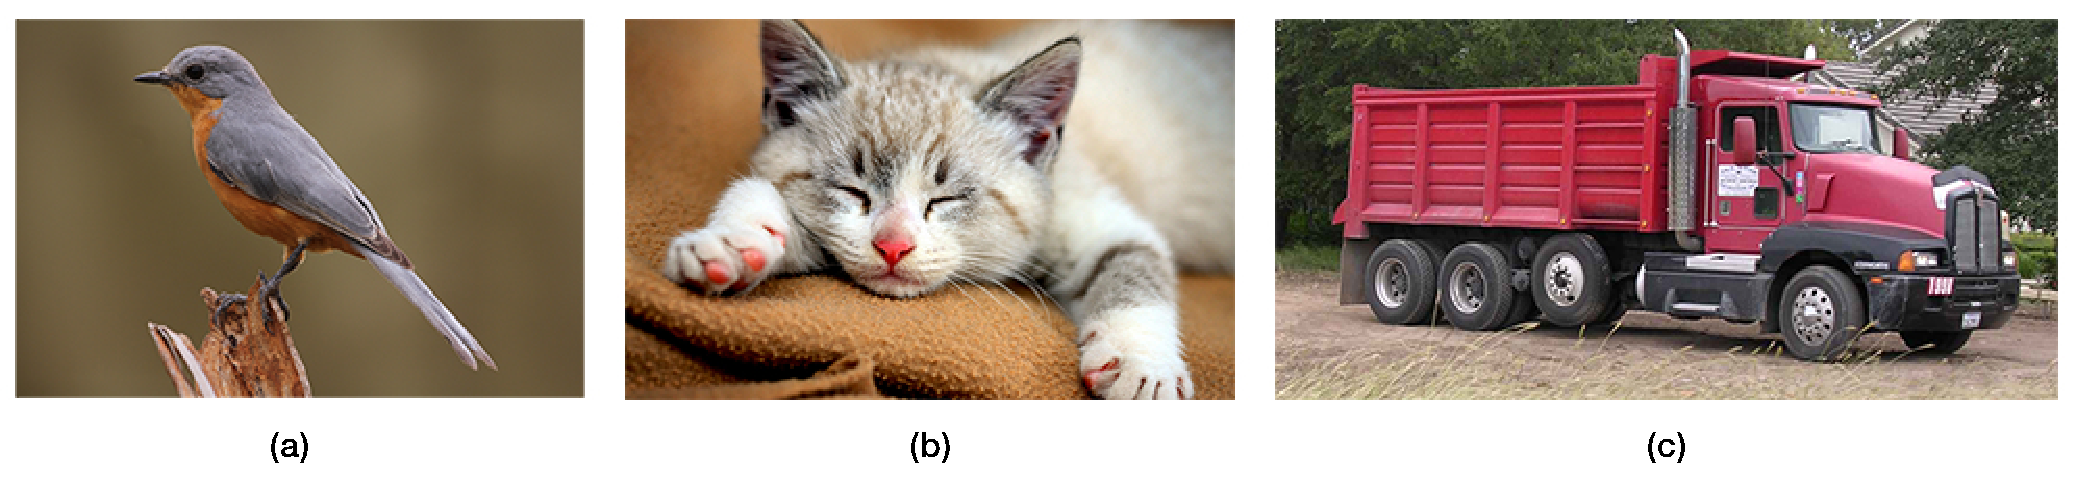
\includegraphics[width=\columnwidth]{Img/classification-images.pdf}
  \caption{Images for classification. The true class of (a) is 'bird', (b) is 'cat', and for (c) is 'truck'. }
  \label{fig:images}
\end{figure}

The python script used for classification of the images is listed in \autoref{lst:script}. The script sets the location of caffe, the image to be classified and the network. The input data is imposed of some preprocessing including reshaping and normalization.

The script then forward passes the image in the network to obtain the classification result. The top 5 labels for the classified image in then printed together with the probability of the images belonging to that label.

\begin{lstlisting}[caption = The python script used for classification with the caffemodel from the original CNN., label={lst:script}]
import numpy as np
import sys
import caffe

# define paths
caffe_root = '../'  # this file is expected to be in {caffe_root}/examples
image = 'examples/images/truck.jpg'

# options
caffe.set_mode_gpu()
net =	caffe.Net(caffe_root + 'models/cifar10/cifar10_quick.prototxt',
        caffe_root + 'models/cifar10/cifar10_quick_iter_4000.caffemodel',
        caffe.TEST)

# input preprocessing
transformer = caffe.io.Transformer({'data': net.blobs['data'].data.shape})
transformer.set_transpose('data', (2,0,1))
# mean pixel
transformer.set_mean('data', np.load(caffe_root + 
					 'models/cifar10/cifar10_mean.npy')
					 .mean(1).mean(1)) 
# the reference model operates on images in [0,255] range instead of [0,1]
transformer.set_raw_scale('data', 255)
# the reference model has channels in BGR order instead of RGB  
transformer.set_channel_swap('data', (2,1,0))  

# do forward pass
net.blobs['data'].data[...] = transformer.preprocess('data', 
							  caffe.io.load_image(caffe_root 
							  + image))
out = net.forward()

# load labels
imagenet_labels_filename = caffe_root + 'data/cifar10/batches.meta.txt'
labels = np.loadtxt(imagenet_labels_filename, str, delimiter='\t')

# sort top 5 predictions from softmax output
top_5 = net.blobs['prob'].data[0].flatten().argsort()[-1:-6:-1]
prob = out['prob'][0]

# print result
for t in top_5:
    print (labels[t] + ": " + str(prob[t]))
\end{lstlisting}

\subsection{Results} % (fold)
\label{sub:results}

The classification result is illustrated in \autoref{fig:images-result}. The class which the image most possibly should be assigned to is the first label. The illustration shows that two out of three images are classified correctly; the bird and the truck. The cat is classified as a ship which is not true class for it.

\begin{figure}[H]
  \centering
  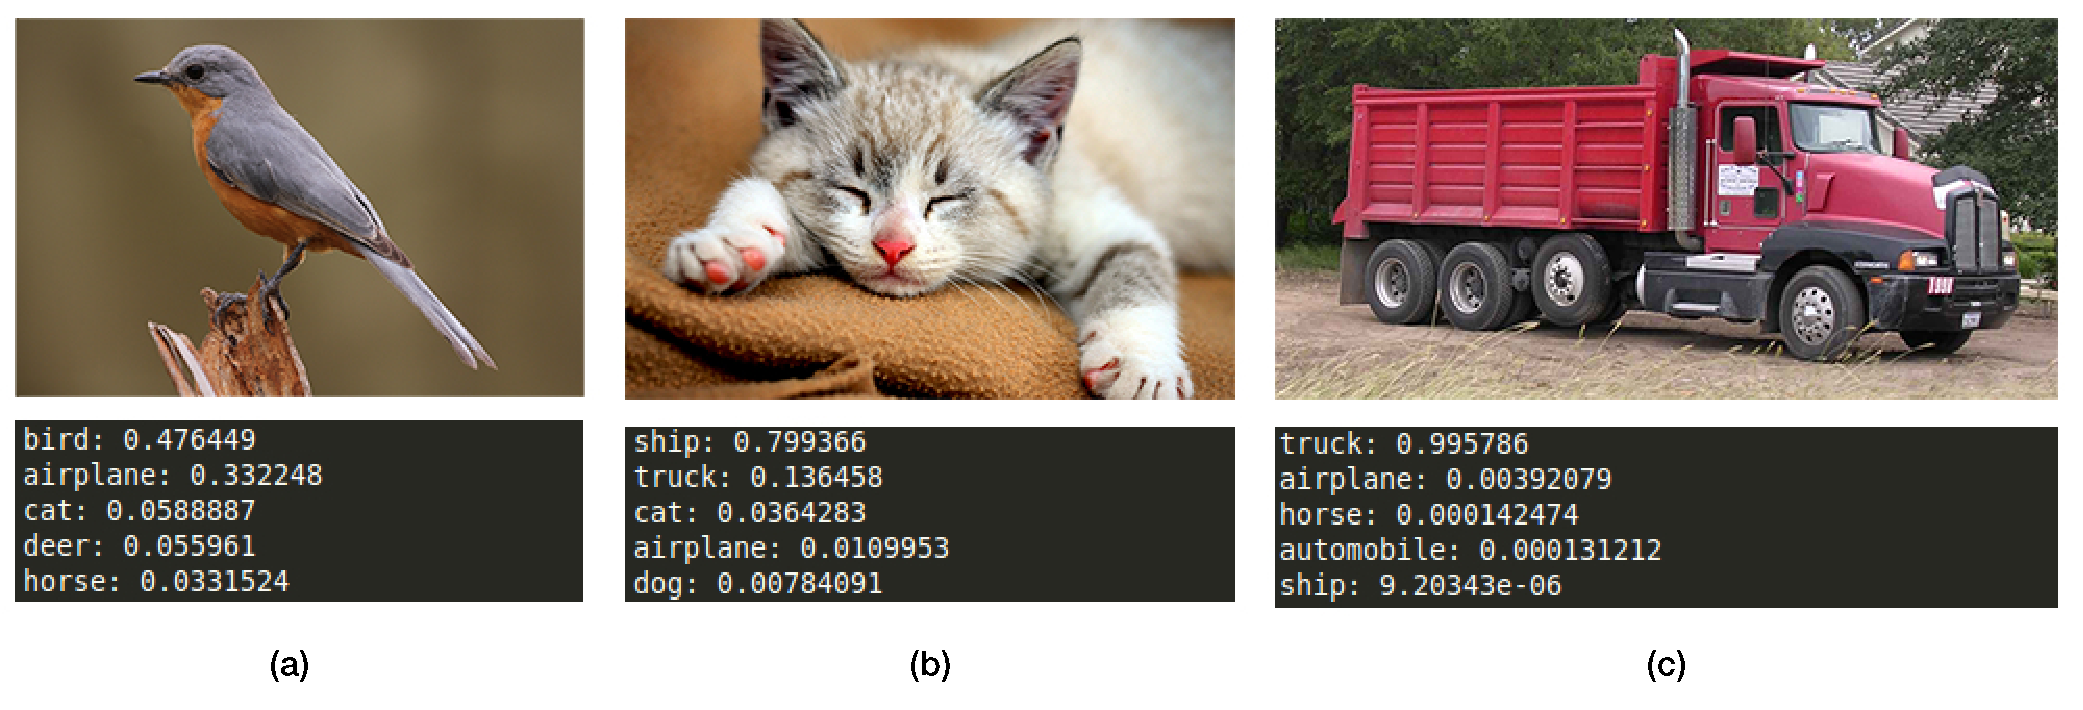
\includegraphics[width=\columnwidth]{Img/classification-images-with-labels.pdf}
  \caption{Result of the classification. The class which the image most possibly should be assigned to is listed af the first label.}
  \label{fig:images-result}
\end{figure}

% subsection results (end)

% section classification (end)